% Created by tikzDevice version 0.10.1 on 2016-12-07 15:45:08
% !TEX encoding = UTF-8 Unicode
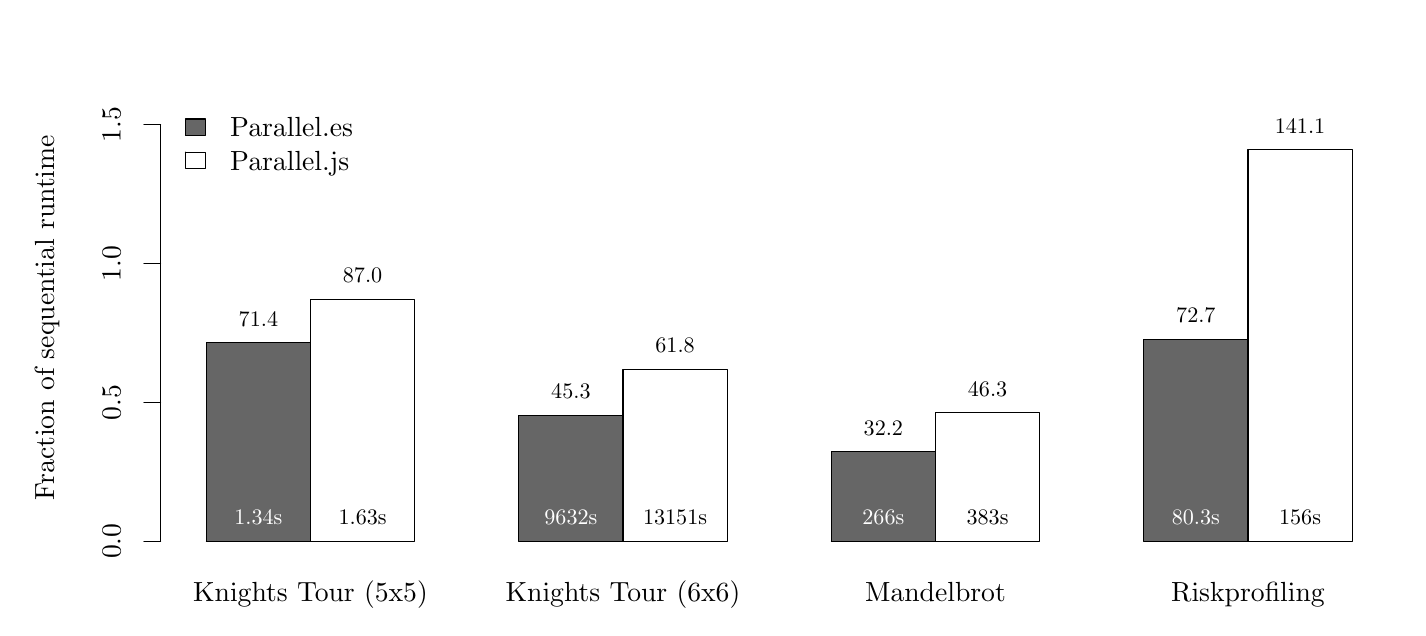
\begin{tikzpicture}[x=1pt,y=1pt]
\definecolor{fillColor}{RGB}{255,255,255}
\path[use as bounding box,fill=fillColor,fill opacity=0.00] (0,0) rectangle (495.15,209.58);
\begin{scope}
\path[clip] (  0.00,  0.00) rectangle (495.15,209.58);
\definecolor{fillColor}{gray}{0.40}

\path[fill=fillColor] ( 64.56, 24.00) --
	(102.20, 24.00) --
	(102.20, 95.67) --
	( 64.56, 95.67) --
	cycle;
\definecolor{drawColor}{RGB}{255,255,255}

\path[draw=drawColor,line width= 0.4pt,line join=round,line cap=round] (102.20,109.50) -- (104.02,111.32);

\path[draw=drawColor,line width= 0.4pt,line join=round,line cap=round] (102.20,106.94) -- (106.58,111.32);

\path[draw=drawColor,line width= 0.4pt,line join=round,line cap=round] (102.20,104.39) -- (109.13,111.32);

\path[draw=drawColor,line width= 0.4pt,line join=round,line cap=round] (102.20,101.83) -- (111.69,111.32);

\path[draw=drawColor,line width= 0.4pt,line join=round,line cap=round] (102.20, 99.28) -- (114.24,111.32);

\path[draw=drawColor,line width= 0.4pt,line join=round,line cap=round] (102.20, 96.72) -- (116.80,111.32);

\path[draw=drawColor,line width= 0.4pt,line join=round,line cap=round] (102.20, 94.17) -- (119.35,111.32);

\path[draw=drawColor,line width= 0.4pt,line join=round,line cap=round] (102.20, 91.61) -- (121.91,111.32);

\path[draw=drawColor,line width= 0.4pt,line join=round,line cap=round] (102.20, 89.06) -- (124.46,111.32);

\path[draw=drawColor,line width= 0.4pt,line join=round,line cap=round] (102.20, 86.50) -- (127.02,111.32);

\path[draw=drawColor,line width= 0.4pt,line join=round,line cap=round] (102.20, 83.95) -- (129.57,111.32);

\path[draw=drawColor,line width= 0.4pt,line join=round,line cap=round] (102.20, 81.39) -- (132.13,111.32);

\path[draw=drawColor,line width= 0.4pt,line join=round,line cap=round] (102.20, 78.84) -- (134.69,111.32);

\path[draw=drawColor,line width= 0.4pt,line join=round,line cap=round] (102.20, 76.28) -- (137.24,111.32);

\path[draw=drawColor,line width= 0.4pt,line join=round,line cap=round] (102.20, 73.73) -- (139.80,111.32);

\path[draw=drawColor,line width= 0.4pt,line join=round,line cap=round] (102.20, 71.17) -- (139.84,108.81);

\path[draw=drawColor,line width= 0.4pt,line join=round,line cap=round] (102.20, 68.62) -- (139.84,106.25);

\path[draw=drawColor,line width= 0.4pt,line join=round,line cap=round] (102.20, 66.06) -- (139.84,103.70);

\path[draw=drawColor,line width= 0.4pt,line join=round,line cap=round] (102.20, 63.51) -- (139.84,101.14);

\path[draw=drawColor,line width= 0.4pt,line join=round,line cap=round] (102.20, 60.95) -- (139.84, 98.59);

\path[draw=drawColor,line width= 0.4pt,line join=round,line cap=round] (102.20, 58.40) -- (139.84, 96.03);

\path[draw=drawColor,line width= 0.4pt,line join=round,line cap=round] (102.20, 55.84) -- (139.84, 93.48);

\path[draw=drawColor,line width= 0.4pt,line join=round,line cap=round] (102.20, 53.28) -- (139.84, 90.92);

\path[draw=drawColor,line width= 0.4pt,line join=round,line cap=round] (102.20, 50.73) -- (139.84, 88.37);

\path[draw=drawColor,line width= 0.4pt,line join=round,line cap=round] (102.20, 48.17) -- (139.84, 85.81);

\path[draw=drawColor,line width= 0.4pt,line join=round,line cap=round] (102.20, 45.62) -- (139.84, 83.26);

\path[draw=drawColor,line width= 0.4pt,line join=round,line cap=round] (102.20, 43.06) -- (139.84, 80.70);

\path[draw=drawColor,line width= 0.4pt,line join=round,line cap=round] (102.20, 40.51) -- (139.84, 78.15);

\path[draw=drawColor,line width= 0.4pt,line join=round,line cap=round] (102.20, 37.95) -- (139.84, 75.59);

\path[draw=drawColor,line width= 0.4pt,line join=round,line cap=round] (102.20, 35.40) -- (139.84, 73.04);

\path[draw=drawColor,line width= 0.4pt,line join=round,line cap=round] (102.20, 32.84) -- (139.84, 70.48);

\path[draw=drawColor,line width= 0.4pt,line join=round,line cap=round] (102.20, 30.29) -- (139.84, 67.93);

\path[draw=drawColor,line width= 0.4pt,line join=round,line cap=round] (102.20, 27.73) -- (139.84, 65.37);

\path[draw=drawColor,line width= 0.4pt,line join=round,line cap=round] (102.20, 25.18) -- (139.84, 62.82);

\path[draw=drawColor,line width= 0.4pt,line join=round,line cap=round] (103.58, 24.00) -- (139.84, 60.26);

\path[draw=drawColor,line width= 0.4pt,line join=round,line cap=round] (106.13, 24.00) -- (139.84, 57.71);

\path[draw=drawColor,line width= 0.4pt,line join=round,line cap=round] (108.69, 24.00) -- (139.84, 55.15);

\path[draw=drawColor,line width= 0.4pt,line join=round,line cap=round] (111.24, 24.00) -- (139.84, 52.60);

\path[draw=drawColor,line width= 0.4pt,line join=round,line cap=round] (113.80, 24.00) -- (139.84, 50.04);

\path[draw=drawColor,line width= 0.4pt,line join=round,line cap=round] (116.35, 24.00) -- (139.84, 47.49);

\path[draw=drawColor,line width= 0.4pt,line join=round,line cap=round] (118.91, 24.00) -- (139.84, 44.93);

\path[draw=drawColor,line width= 0.4pt,line join=round,line cap=round] (121.46, 24.00) -- (139.84, 42.38);

\path[draw=drawColor,line width= 0.4pt,line join=round,line cap=round] (124.02, 24.00) -- (139.84, 39.82);

\path[draw=drawColor,line width= 0.4pt,line join=round,line cap=round] (126.57, 24.00) -- (139.84, 37.27);

\path[draw=drawColor,line width= 0.4pt,line join=round,line cap=round] (129.13, 24.00) -- (139.84, 34.71);

\path[draw=drawColor,line width= 0.4pt,line join=round,line cap=round] (131.68, 24.00) -- (139.84, 32.16);

\path[draw=drawColor,line width= 0.4pt,line join=round,line cap=round] (134.24, 24.00) -- (139.84, 29.60);

\path[draw=drawColor,line width= 0.4pt,line join=round,line cap=round] (136.79, 24.00) -- (139.84, 27.05);

\path[draw=drawColor,line width= 0.4pt,line join=round,line cap=round] (139.35, 24.00) -- (139.84, 24.49);

\path[fill=fillColor] (177.48, 24.00) --
	(215.12, 24.00) --
	(215.12, 69.43) --
	(177.48, 69.43) --
	cycle;

\path[draw=drawColor,line width= 0.4pt,line join=round,line cap=round] (215.12, 84.44) -- (216.70, 86.03);

\path[draw=drawColor,line width= 0.4pt,line join=round,line cap=round] (215.12, 81.88) -- (219.26, 86.03);

\path[draw=drawColor,line width= 0.4pt,line join=round,line cap=round] (215.12, 79.33) -- (221.81, 86.03);

\path[draw=drawColor,line width= 0.4pt,line join=round,line cap=round] (215.12, 76.77) -- (224.37, 86.03);

\path[draw=drawColor,line width= 0.4pt,line join=round,line cap=round] (215.12, 74.22) -- (226.92, 86.03);

\path[draw=drawColor,line width= 0.4pt,line join=round,line cap=round] (215.12, 71.66) -- (229.48, 86.03);

\path[draw=drawColor,line width= 0.4pt,line join=round,line cap=round] (215.12, 69.11) -- (232.03, 86.03);

\path[draw=drawColor,line width= 0.4pt,line join=round,line cap=round] (215.12, 66.55) -- (234.59, 86.03);

\path[draw=drawColor,line width= 0.4pt,line join=round,line cap=round] (215.12, 64.00) -- (237.15, 86.03);

\path[draw=drawColor,line width= 0.4pt,line join=round,line cap=round] (215.12, 61.44) -- (239.70, 86.03);

\path[draw=drawColor,line width= 0.4pt,line join=round,line cap=round] (215.12, 58.89) -- (242.26, 86.03);

\path[draw=drawColor,line width= 0.4pt,line join=round,line cap=round] (215.12, 56.33) -- (244.81, 86.03);

\path[draw=drawColor,line width= 0.4pt,line join=round,line cap=round] (215.12, 53.78) -- (247.37, 86.03);

\path[draw=drawColor,line width= 0.4pt,line join=round,line cap=round] (215.12, 51.22) -- (249.92, 86.03);

\path[draw=drawColor,line width= 0.4pt,line join=round,line cap=round] (215.12, 48.66) -- (252.48, 86.03);

\path[draw=drawColor,line width= 0.4pt,line join=round,line cap=round] (215.12, 46.11) -- (252.75, 83.75);

\path[draw=drawColor,line width= 0.4pt,line join=round,line cap=round] (215.12, 43.55) -- (252.75, 81.19);

\path[draw=drawColor,line width= 0.4pt,line join=round,line cap=round] (215.12, 41.00) -- (252.75, 78.64);

\path[draw=drawColor,line width= 0.4pt,line join=round,line cap=round] (215.12, 38.44) -- (252.75, 76.08);

\path[draw=drawColor,line width= 0.4pt,line join=round,line cap=round] (215.12, 35.89) -- (252.75, 73.53);

\path[draw=drawColor,line width= 0.4pt,line join=round,line cap=round] (215.12, 33.33) -- (252.75, 70.97);

\path[draw=drawColor,line width= 0.4pt,line join=round,line cap=round] (215.12, 30.78) -- (252.75, 68.42);

\path[draw=drawColor,line width= 0.4pt,line join=round,line cap=round] (215.12, 28.22) -- (252.75, 65.86);

\path[draw=drawColor,line width= 0.4pt,line join=round,line cap=round] (215.12, 25.67) -- (252.75, 63.31);

\path[draw=drawColor,line width= 0.4pt,line join=round,line cap=round] (216.00, 24.00) -- (252.75, 60.75);

\path[draw=drawColor,line width= 0.4pt,line join=round,line cap=round] (218.56, 24.00) -- (252.75, 58.20);

\path[draw=drawColor,line width= 0.4pt,line join=round,line cap=round] (221.11, 24.00) -- (252.75, 55.64);

\path[draw=drawColor,line width= 0.4pt,line join=round,line cap=round] (223.67, 24.00) -- (252.75, 53.09);

\path[draw=drawColor,line width= 0.4pt,line join=round,line cap=round] (226.22, 24.00) -- (252.75, 50.53);

\path[draw=drawColor,line width= 0.4pt,line join=round,line cap=round] (228.78, 24.00) -- (252.75, 47.98);

\path[draw=drawColor,line width= 0.4pt,line join=round,line cap=round] (231.33, 24.00) -- (252.75, 45.42);

\path[draw=drawColor,line width= 0.4pt,line join=round,line cap=round] (233.89, 24.00) -- (252.75, 42.87);

\path[draw=drawColor,line width= 0.4pt,line join=round,line cap=round] (236.44, 24.00) -- (252.75, 40.31);

\path[draw=drawColor,line width= 0.4pt,line join=round,line cap=round] (239.00, 24.00) -- (252.75, 37.76);

\path[draw=drawColor,line width= 0.4pt,line join=round,line cap=round] (241.55, 24.00) -- (252.75, 35.20);

\path[draw=drawColor,line width= 0.4pt,line join=round,line cap=round] (244.11, 24.00) -- (252.75, 32.65);

\path[draw=drawColor,line width= 0.4pt,line join=round,line cap=round] (246.66, 24.00) -- (252.75, 30.09);

\path[draw=drawColor,line width= 0.4pt,line join=round,line cap=round] (249.22, 24.00) -- (252.75, 27.54);

\path[draw=drawColor,line width= 0.4pt,line join=round,line cap=round] (251.77, 24.00) -- (252.75, 24.98);

\path[fill=fillColor] (290.39, 24.00) --
	(328.03, 24.00) --
	(328.03, 56.27) --
	(290.39, 56.27) --
	cycle;

\path[draw=drawColor,line width= 0.4pt,line join=round,line cap=round] (328.03, 69.60) -- (328.89, 70.45);

\path[draw=drawColor,line width= 0.4pt,line join=round,line cap=round] (328.03, 67.04) -- (331.44, 70.45);

\path[draw=drawColor,line width= 0.4pt,line join=round,line cap=round] (328.03, 64.49) -- (334.00, 70.45);

\path[draw=drawColor,line width= 0.4pt,line join=round,line cap=round] (328.03, 61.93) -- (336.55, 70.45);

\path[draw=drawColor,line width= 0.4pt,line join=round,line cap=round] (328.03, 59.38) -- (339.11, 70.45);

\path[draw=drawColor,line width= 0.4pt,line join=round,line cap=round] (328.03, 56.82) -- (341.66, 70.45);

\path[draw=drawColor,line width= 0.4pt,line join=round,line cap=round] (328.03, 54.27) -- (344.22, 70.45);

\path[draw=drawColor,line width= 0.4pt,line join=round,line cap=round] (328.03, 51.71) -- (346.77, 70.45);

\path[draw=drawColor,line width= 0.4pt,line join=round,line cap=round] (328.03, 49.16) -- (349.33, 70.45);

\path[draw=drawColor,line width= 0.4pt,line join=round,line cap=round] (328.03, 46.60) -- (351.88, 70.45);

\path[draw=drawColor,line width= 0.4pt,line join=round,line cap=round] (328.03, 44.04) -- (354.44, 70.45);

\path[draw=drawColor,line width= 0.4pt,line join=round,line cap=round] (328.03, 41.49) -- (356.99, 70.45);

\path[draw=drawColor,line width= 0.4pt,line join=round,line cap=round] (328.03, 38.93) -- (359.55, 70.45);

\path[draw=drawColor,line width= 0.4pt,line join=round,line cap=round] (328.03, 36.38) -- (362.10, 70.45);

\path[draw=drawColor,line width= 0.4pt,line join=round,line cap=round] (328.03, 33.82) -- (364.66, 70.45);

\path[draw=drawColor,line width= 0.4pt,line join=round,line cap=round] (328.03, 31.27) -- (365.67, 68.91);

\path[draw=drawColor,line width= 0.4pt,line join=round,line cap=round] (328.03, 28.71) -- (365.67, 66.35);

\path[draw=drawColor,line width= 0.4pt,line join=round,line cap=round] (328.03, 26.16) -- (365.67, 63.80);

\path[draw=drawColor,line width= 0.4pt,line join=round,line cap=round] (328.43, 24.00) -- (365.67, 61.24);

\path[draw=drawColor,line width= 0.4pt,line join=round,line cap=round] (330.98, 24.00) -- (365.67, 58.69);

\path[draw=drawColor,line width= 0.4pt,line join=round,line cap=round] (333.54, 24.00) -- (365.67, 56.13);

\path[draw=drawColor,line width= 0.4pt,line join=round,line cap=round] (336.09, 24.00) -- (365.67, 53.58);

\path[draw=drawColor,line width= 0.4pt,line join=round,line cap=round] (338.65, 24.00) -- (365.67, 51.02);

\path[draw=drawColor,line width= 0.4pt,line join=round,line cap=round] (341.20, 24.00) -- (365.67, 48.47);

\path[draw=drawColor,line width= 0.4pt,line join=round,line cap=round] (343.76, 24.00) -- (365.67, 45.91);

\path[draw=drawColor,line width= 0.4pt,line join=round,line cap=round] (346.31, 24.00) -- (365.67, 43.36);

\path[draw=drawColor,line width= 0.4pt,line join=round,line cap=round] (348.87, 24.00) -- (365.67, 40.80);

\path[draw=drawColor,line width= 0.4pt,line join=round,line cap=round] (351.42, 24.00) -- (365.67, 38.25);

\path[draw=drawColor,line width= 0.4pt,line join=round,line cap=round] (353.98, 24.00) -- (365.67, 35.69);

\path[draw=drawColor,line width= 0.4pt,line join=round,line cap=round] (356.53, 24.00) -- (365.67, 33.14);

\path[draw=drawColor,line width= 0.4pt,line join=round,line cap=round] (359.09, 24.00) -- (365.67, 30.58);

\path[draw=drawColor,line width= 0.4pt,line join=round,line cap=round] (361.64, 24.00) -- (365.67, 28.03);

\path[draw=drawColor,line width= 0.4pt,line join=round,line cap=round] (364.20, 24.00) -- (365.67, 25.47);

\path[fill=fillColor] (403.31, 24.00) --
	(440.95, 24.00) --
	(440.95, 96.94) --
	(403.31, 96.94) --
	cycle;

\path[draw=drawColor,line width= 0.4pt,line join=round,line cap=round] (440.95,164.63) -- (441.84,165.52);

\path[draw=drawColor,line width= 0.4pt,line join=round,line cap=round] (440.95,162.07) -- (444.40,165.52);

\path[draw=drawColor,line width= 0.4pt,line join=round,line cap=round] (440.95,159.52) -- (446.95,165.52);

\path[draw=drawColor,line width= 0.4pt,line join=round,line cap=round] (440.95,156.96) -- (449.51,165.52);

\path[draw=drawColor,line width= 0.4pt,line join=round,line cap=round] (440.95,154.41) -- (452.06,165.52);

\path[draw=drawColor,line width= 0.4pt,line join=round,line cap=round] (440.95,151.85) -- (454.62,165.52);

\path[draw=drawColor,line width= 0.4pt,line join=round,line cap=round] (440.95,149.30) -- (457.17,165.52);

\path[draw=drawColor,line width= 0.4pt,line join=round,line cap=round] (440.95,146.74) -- (459.73,165.52);

\path[draw=drawColor,line width= 0.4pt,line join=round,line cap=round] (440.95,144.19) -- (462.28,165.52);

\path[draw=drawColor,line width= 0.4pt,line join=round,line cap=round] (440.95,141.63) -- (464.84,165.52);

\path[draw=drawColor,line width= 0.4pt,line join=round,line cap=round] (440.95,139.07) -- (467.39,165.52);

\path[draw=drawColor,line width= 0.4pt,line join=round,line cap=round] (440.95,136.52) -- (469.95,165.52);

\path[draw=drawColor,line width= 0.4pt,line join=round,line cap=round] (440.95,133.96) -- (472.50,165.52);

\path[draw=drawColor,line width= 0.4pt,line join=round,line cap=round] (440.95,131.41) -- (475.06,165.52);

\path[draw=drawColor,line width= 0.4pt,line join=round,line cap=round] (440.95,128.85) -- (477.61,165.52);

\path[draw=drawColor,line width= 0.4pt,line join=round,line cap=round] (440.95,126.30) -- (478.59,163.94);

\path[draw=drawColor,line width= 0.4pt,line join=round,line cap=round] (440.95,123.74) -- (478.59,161.38);

\path[draw=drawColor,line width= 0.4pt,line join=round,line cap=round] (440.95,121.19) -- (478.59,158.83);

\path[draw=drawColor,line width= 0.4pt,line join=round,line cap=round] (440.95,118.63) -- (478.59,156.27);

\path[draw=drawColor,line width= 0.4pt,line join=round,line cap=round] (440.95,116.08) -- (478.59,153.72);

\path[draw=drawColor,line width= 0.4pt,line join=round,line cap=round] (440.95,113.52) -- (478.59,151.16);

\path[draw=drawColor,line width= 0.4pt,line join=round,line cap=round] (440.95,110.97) -- (478.59,148.61);

\path[draw=drawColor,line width= 0.4pt,line join=round,line cap=round] (440.95,108.41) -- (478.59,146.05);

\path[draw=drawColor,line width= 0.4pt,line join=round,line cap=round] (440.95,105.86) -- (478.59,143.50);

\path[draw=drawColor,line width= 0.4pt,line join=round,line cap=round] (440.95,103.30) -- (478.59,140.94);

\path[draw=drawColor,line width= 0.4pt,line join=round,line cap=round] (440.95,100.75) -- (478.59,138.39);

\path[draw=drawColor,line width= 0.4pt,line join=round,line cap=round] (440.95, 98.19) -- (478.59,135.83);

\path[draw=drawColor,line width= 0.4pt,line join=round,line cap=round] (440.95, 95.64) -- (478.59,133.28);

\path[draw=drawColor,line width= 0.4pt,line join=round,line cap=round] (440.95, 93.08) -- (478.59,130.72);

\path[draw=drawColor,line width= 0.4pt,line join=round,line cap=round] (440.95, 90.53) -- (478.59,128.17);

\path[draw=drawColor,line width= 0.4pt,line join=round,line cap=round] (440.95, 87.97) -- (478.59,125.61);

\path[draw=drawColor,line width= 0.4pt,line join=round,line cap=round] (440.95, 85.42) -- (478.59,123.06);

\path[draw=drawColor,line width= 0.4pt,line join=round,line cap=round] (440.95, 82.86) -- (478.59,120.50);

\path[draw=drawColor,line width= 0.4pt,line join=round,line cap=round] (440.95, 80.31) -- (478.59,117.95);

\path[draw=drawColor,line width= 0.4pt,line join=round,line cap=round] (440.95, 77.75) -- (478.59,115.39);

\path[draw=drawColor,line width= 0.4pt,line join=round,line cap=round] (440.95, 75.20) -- (478.59,112.84);

\path[draw=drawColor,line width= 0.4pt,line join=round,line cap=round] (440.95, 72.64) -- (478.59,110.28);

\path[draw=drawColor,line width= 0.4pt,line join=round,line cap=round] (440.95, 70.09) -- (478.59,107.72);

\path[draw=drawColor,line width= 0.4pt,line join=round,line cap=round] (440.95, 67.53) -- (478.59,105.17);

\path[draw=drawColor,line width= 0.4pt,line join=round,line cap=round] (440.95, 64.98) -- (478.59,102.61);

\path[draw=drawColor,line width= 0.4pt,line join=round,line cap=round] (440.95, 62.42) -- (478.59,100.06);

\path[draw=drawColor,line width= 0.4pt,line join=round,line cap=round] (440.95, 59.87) -- (478.59, 97.50);

\path[draw=drawColor,line width= 0.4pt,line join=round,line cap=round] (440.95, 57.31) -- (478.59, 94.95);

\path[draw=drawColor,line width= 0.4pt,line join=round,line cap=round] (440.95, 54.76) -- (478.59, 92.39);

\path[draw=drawColor,line width= 0.4pt,line join=round,line cap=round] (440.95, 52.20) -- (478.59, 89.84);

\path[draw=drawColor,line width= 0.4pt,line join=round,line cap=round] (440.95, 49.65) -- (478.59, 87.28);

\path[draw=drawColor,line width= 0.4pt,line join=round,line cap=round] (440.95, 47.09) -- (478.59, 84.73);

\path[draw=drawColor,line width= 0.4pt,line join=round,line cap=round] (440.95, 44.53) -- (478.59, 82.17);

\path[draw=drawColor,line width= 0.4pt,line join=round,line cap=round] (440.95, 41.98) -- (478.59, 79.62);

\path[draw=drawColor,line width= 0.4pt,line join=round,line cap=round] (440.95, 39.42) -- (478.59, 77.06);

\path[draw=drawColor,line width= 0.4pt,line join=round,line cap=round] (440.95, 36.87) -- (478.59, 74.51);

\path[draw=drawColor,line width= 0.4pt,line join=round,line cap=round] (440.95, 34.31) -- (478.59, 71.95);

\path[draw=drawColor,line width= 0.4pt,line join=round,line cap=round] (440.95, 31.76) -- (478.59, 69.40);

\path[draw=drawColor,line width= 0.4pt,line join=round,line cap=round] (440.95, 29.20) -- (478.59, 66.84);

\path[draw=drawColor,line width= 0.4pt,line join=round,line cap=round] (440.95, 26.65) -- (478.59, 64.29);

\path[draw=drawColor,line width= 0.4pt,line join=round,line cap=round] (440.95, 24.09) -- (478.59, 61.73);

\path[draw=drawColor,line width= 0.4pt,line join=round,line cap=round] (443.41, 24.00) -- (478.59, 59.18);

\path[draw=drawColor,line width= 0.4pt,line join=round,line cap=round] (445.96, 24.00) -- (478.59, 56.62);

\path[draw=drawColor,line width= 0.4pt,line join=round,line cap=round] (448.52, 24.00) -- (478.59, 54.07);

\path[draw=drawColor,line width= 0.4pt,line join=round,line cap=round] (451.07, 24.00) -- (478.59, 51.51);

\path[draw=drawColor,line width= 0.4pt,line join=round,line cap=round] (453.63, 24.00) -- (478.59, 48.96);

\path[draw=drawColor,line width= 0.4pt,line join=round,line cap=round] (456.18, 24.00) -- (478.59, 46.40);

\path[draw=drawColor,line width= 0.4pt,line join=round,line cap=round] (458.74, 24.00) -- (478.59, 43.85);

\path[draw=drawColor,line width= 0.4pt,line join=round,line cap=round] (461.29, 24.00) -- (478.59, 41.29);

\path[draw=drawColor,line width= 0.4pt,line join=round,line cap=round] (463.85, 24.00) -- (478.59, 38.74);

\path[draw=drawColor,line width= 0.4pt,line join=round,line cap=round] (466.40, 24.00) -- (478.59, 36.18);

\path[draw=drawColor,line width= 0.4pt,line join=round,line cap=round] (468.96, 24.00) -- (478.59, 33.63);

\path[draw=drawColor,line width= 0.4pt,line join=round,line cap=round] (471.52, 24.00) -- (478.59, 31.07);

\path[draw=drawColor,line width= 0.4pt,line join=round,line cap=round] (474.07, 24.00) -- (478.59, 28.52);

\path[draw=drawColor,line width= 0.4pt,line join=round,line cap=round] (476.63, 24.00) -- (478.59, 25.96);
\definecolor{drawColor}{RGB}{0,0,0}

\path[draw=drawColor,line width= 0.4pt,line join=round,line cap=round] ( 64.56, 24.00) --
	(102.20, 24.00) --
	(102.20, 95.67) --
	( 64.56, 95.67) --
	( 64.56, 24.00);

\path[draw=drawColor,line width= 0.4pt,line join=round,line cap=round] (102.20, 24.00) --
	(139.84, 24.00) --
	(139.84,111.32) --
	(102.20,111.32) --
	(102.20, 24.00);

\path[draw=drawColor,line width= 0.4pt,line join=round,line cap=round] (177.48, 24.00) --
	(215.12, 24.00) --
	(215.12, 69.43) --
	(177.48, 69.43) --
	(177.48, 24.00);

\path[draw=drawColor,line width= 0.4pt,line join=round,line cap=round] (215.12, 24.00) --
	(252.75, 24.00) --
	(252.75, 86.03) --
	(215.12, 86.03) --
	(215.12, 24.00);

\path[draw=drawColor,line width= 0.4pt,line join=round,line cap=round] (290.39, 24.00) --
	(328.03, 24.00) --
	(328.03, 56.27) --
	(290.39, 56.27) --
	(290.39, 24.00);

\path[draw=drawColor,line width= 0.4pt,line join=round,line cap=round] (328.03, 24.00) --
	(365.67, 24.00) --
	(365.67, 70.45) --
	(328.03, 70.45) --
	(328.03, 24.00);

\path[draw=drawColor,line width= 0.4pt,line join=round,line cap=round] (403.31, 24.00) --
	(440.95, 24.00) --
	(440.95, 96.94) --
	(403.31, 96.94) --
	(403.31, 24.00);

\path[draw=drawColor,line width= 0.4pt,line join=round,line cap=round] (440.95, 24.00) --
	(478.59, 24.00) --
	(478.59,165.52) --
	(440.95,165.52) --
	(440.95, 24.00);
\end{scope}
\begin{scope}
\path[clip] (  0.00,  0.00) rectangle (495.15,209.58);
\definecolor{drawColor}{RGB}{0,0,0}

\node[text=drawColor,anchor=base,inner sep=0pt, outer sep=0pt, scale=  1.00] at (102.20,  2.40) {Knights Tour (5x5)};

\node[text=drawColor,anchor=base,inner sep=0pt, outer sep=0pt, scale=  1.00] at (215.12,  2.40) {Knights Tour (6x6)};

\node[text=drawColor,anchor=base,inner sep=0pt, outer sep=0pt, scale=  1.00] at (328.03,  2.40) {Mandelbrot};

\node[text=drawColor,anchor=base,inner sep=0pt, outer sep=0pt, scale=  1.00] at (440.95,  2.40) {Riskprofiling};
\end{scope}
\begin{scope}
\path[clip] (  0.00,  0.00) rectangle (495.15,209.58);
\definecolor{drawColor}{RGB}{0,0,0}

\node[text=drawColor,rotate= 90.00,anchor=base,inner sep=0pt, outer sep=0pt, scale=  1.00] at (  9.60,104.79) {Fraction of sequential runtime};
\end{scope}
\begin{scope}
\path[clip] (  0.00,  0.00) rectangle (495.15,209.58);
\definecolor{drawColor}{RGB}{0,0,0}

\path[draw=drawColor,line width= 0.4pt,line join=round,line cap=round] ( 48.00, 24.00) -- ( 48.00,174.48);

\path[draw=drawColor,line width= 0.4pt,line join=round,line cap=round] ( 48.00, 24.00) -- ( 42.00, 24.00);

\path[draw=drawColor,line width= 0.4pt,line join=round,line cap=round] ( 48.00, 74.16) -- ( 42.00, 74.16);

\path[draw=drawColor,line width= 0.4pt,line join=round,line cap=round] ( 48.00,124.32) -- ( 42.00,124.32);

\path[draw=drawColor,line width= 0.4pt,line join=round,line cap=round] ( 48.00,174.48) -- ( 42.00,174.48);

\node[text=drawColor,rotate= 90.00,anchor=base,inner sep=0pt, outer sep=0pt, scale=  1.00] at ( 33.60, 24.00) {0.0};

\node[text=drawColor,rotate= 90.00,anchor=base,inner sep=0pt, outer sep=0pt, scale=  1.00] at ( 33.60, 74.16) {0.5};

\node[text=drawColor,rotate= 90.00,anchor=base,inner sep=0pt, outer sep=0pt, scale=  1.00] at ( 33.60,124.32) {1.0};

\node[text=drawColor,rotate= 90.00,anchor=base,inner sep=0pt, outer sep=0pt, scale=  1.00] at ( 33.60,174.48) {1.5};
\end{scope}
\begin{scope}
\path[clip] ( 48.00, 24.00) rectangle (495.15,185.58);
\definecolor{fillColor}{gray}{0.40}

\path[fill=fillColor] ( 57.00,176.58) --
	( 64.20,176.58) --
	( 64.20,170.58) --
	( 57.00,170.58) --
	cycle;
\definecolor{drawColor}{RGB}{255,255,255}

\path[draw=drawColor,line width= 0.4pt,line join=round,line cap=round] ( 57.00,163.95) -- ( 57.63,164.58);

\path[draw=drawColor,line width= 0.4pt,line join=round,line cap=round] ( 57.00,161.39) -- ( 60.19,164.58);

\path[draw=drawColor,line width= 0.4pt,line join=round,line cap=round] ( 57.00,158.84) -- ( 62.75,164.58);

\path[draw=drawColor,line width= 0.4pt,line join=round,line cap=round] ( 59.30,158.58) -- ( 64.20,163.48);

\path[draw=drawColor,line width= 0.4pt,line join=round,line cap=round] ( 61.86,158.58) -- ( 64.20,160.93);
\definecolor{drawColor}{RGB}{0,0,0}

\path[draw=drawColor,line width= 0.4pt,line join=round,line cap=round] ( 57.00,176.58) --
	( 64.20,176.58) --
	( 64.20,170.58) --
	( 57.00,170.58) --
	( 57.00,176.58);

\path[draw=drawColor,line width= 0.4pt,line join=round,line cap=round] ( 57.00,164.58) --
	( 64.20,164.58) --
	( 64.20,158.58) --
	( 57.00,158.58) --
	( 57.00,164.58);

\node[text=drawColor,anchor=base west,inner sep=0pt, outer sep=0pt, scale=  1.00] at ( 73.20,170.14) {Parallel.es};

\node[text=drawColor,anchor=base west,inner sep=0pt, outer sep=0pt, scale=  1.00] at ( 73.20,158.14) {Parallel.js};

\node[text=drawColor,anchor=base,inner sep=0pt, outer sep=0pt, scale=  0.80] at ( 83.38,101.67) {71.4};

\node[text=drawColor,anchor=base,inner sep=0pt, outer sep=0pt, scale=  0.80] at (121.02,117.32) {87.0};

\node[text=drawColor,anchor=base,inner sep=0pt, outer sep=0pt, scale=  0.80] at (196.30, 75.43) {45.3};

\node[text=drawColor,anchor=base,inner sep=0pt, outer sep=0pt, scale=  0.80] at (233.93, 92.03) {61.8};

\node[text=drawColor,anchor=base,inner sep=0pt, outer sep=0pt, scale=  0.80] at (309.21, 62.27) {32.2};

\node[text=drawColor,anchor=base,inner sep=0pt, outer sep=0pt, scale=  0.80] at (346.85, 76.45) {46.3};

\node[text=drawColor,anchor=base,inner sep=0pt, outer sep=0pt, scale=  0.80] at (422.13,102.94) {72.7};

\node[text=drawColor,anchor=base,inner sep=0pt, outer sep=0pt, scale=  0.80] at (459.77,171.52) {141.1};
\definecolor{drawColor}{RGB}{255,255,255}

\node[text=drawColor,anchor=base,inner sep=0pt, outer sep=0pt, scale=  0.80] at ( 83.38, 30.00) {1.34s};
\definecolor{drawColor}{RGB}{0,0,0}

\node[text=drawColor,anchor=base,inner sep=0pt, outer sep=0pt, scale=  0.80] at (121.02, 30.00) {1.63s};
\definecolor{drawColor}{RGB}{255,255,255}

\node[text=drawColor,anchor=base,inner sep=0pt, outer sep=0pt, scale=  0.80] at (196.30, 30.00) {9632s};
\definecolor{drawColor}{RGB}{0,0,0}

\node[text=drawColor,anchor=base,inner sep=0pt, outer sep=0pt, scale=  0.80] at (233.93, 30.00) {13151s};
\definecolor{drawColor}{RGB}{255,255,255}

\node[text=drawColor,anchor=base,inner sep=0pt, outer sep=0pt, scale=  0.80] at (309.21, 30.00) {266s};
\definecolor{drawColor}{RGB}{0,0,0}

\node[text=drawColor,anchor=base,inner sep=0pt, outer sep=0pt, scale=  0.80] at (346.85, 30.00) {383s};
\definecolor{drawColor}{RGB}{255,255,255}

\node[text=drawColor,anchor=base,inner sep=0pt, outer sep=0pt, scale=  0.80] at (422.13, 30.00) {80.3s};
\definecolor{drawColor}{RGB}{0,0,0}

\node[text=drawColor,anchor=base,inner sep=0pt, outer sep=0pt, scale=  0.80] at (459.77, 30.00) {156s};
\end{scope}
\end{tikzpicture}
